\section{Introduction}

The advent of Generative Adversarial Networks (GANs) has brought with it a renaissance in the field of content creation and manipulation, allowing users to modify photographs in intuitive ways. In particular, the highly disentangled latent space of StyleGAN \cite{karras2019style,karras2020analyzing} has been widely adapted for realistic editing of facial images. However, these semantic editing tools have been mostly restricted to images, as the editing of videos imposes an additional challenge -- maintaining \textit{temporal coherency}. Any manipulation of the video must be propagated consistently across all video frames. Prior work suggests tackling this challenge by training a GAN for video synthesis~\cite{skorokhodov2021stylegan,yan2021videogpt,yu2022generating}. However, with a lack of high quality video datasets and the complications arising from an additional data dimension, video-GANs have so far been unable to match the quality of their single-image counterparts. 

Instead, we propose to meet this challenge by using the latent-editing techniques commonly employed with an off-the-shelf, non-temporal StyleGAN model.
%, and without additional supervision.
We highlight a fundamental assumption about the video editing process: the initial video is already consistent. In contrast to synthesis works, we do not need to \textit{create} temporal consistency, but only \textit{maintain} it. Building on this intuition, we revisit the building blocks of recent StyleGAN-based editing pipelines, identify the points where temporal inconsistencies may arise, and propose that in many cases these inconsistencies can be mitigated simply through a careful choice of tools. 
%\ron{By exploiting the natural smoothness of neural networks, we successfully perform temporally consistent semantic editing.}

We begin our investigation by identifying two types of temporal inconsistencies: local -- where the transitions between adjacent frames are not smooth and display considerable jitter, and global -- where inaccuracies in the GAN editing process, such as changes in identity, build up over time.
We consider the recently proposed PTI~\cite{roich2021pivotal}; A two-step approach to inversion which first finds a 'pivot' -- an initial latent code that can be fed through the generator to produce an approximation of the input image. Then, the generator's weights are fine-tuned so that the specific 'pivot' code can better reproduce the target. PTI provides strong global consistency, keeping the identity aligned with the target video. However, our investigation reveals that it fares poorly on the local benchmark and produces inversions which behave inconsistently under editing operations.

At this point, we make two key observations: The generator is a highly parametric neural function, which are known to be predisposed to learning low frequency functions. As such, a small change in its inputs (the latent codes) is likely to induce only a minor variation in the generated images. Moreover, it has been shown that style-based models maintain incredible alignment under fine-tuning, particularly when transitioning to nearby domains \cite{wu2021stylealign,pinkney2020resolution,gal2021stylegannada}. As such, if the generator produces consistent editing for a set of smoothly changing latent codes - we expect any fine-tuned generator to be similarly predisposed towards temporal consistency. 

With these intuitions in mind, we propose that PTI's local inconsistency arises at the first step of the process -- finding the 'pivots'. More specifically, the employed optimization-based inversion is inconsistent. Highly similar frames can be encoded into different regions of the latent space, even when using the same initialization and random noise seed. On the other hand, encoder-based inversion methods utilize highly parametrized networks, and are therefore also biased to low-frequency representations. As such, an encoder is likely to provide slowly changing latents when its input only undergoes a minor change - such as when observing two adjacent video frames.

We merge the two approaches: an encoder for discovering locally consistent pivots, and generator fine-tuning to promote global consistency, and demonstrate that they already provide a strongly consistent prior.
Nevertheless, they are not sufficient for editing real videos. As StyleGAN cannot operate over the entire frame, we need to stitch the edited crop back to the original video. However, inversion and editing methods typically corrupt the background extensively, making their results difficult to blend into the original frame. For this purpose, we design a novel `stitching-tuning' operation that further tunes the generator to provide spatially-consistent transitions. By doing so, we achieve realistic blending while retaining the editing effects.

We demonstrate that our proposed editing pipeline can seamlessly apply latent-based semantic modifications to faces in real videos. Although we employ only non-temporal models, we can successfully edit challenging talking head videos with considerable movement and complex backgrounds, which current methods fail to tackle. In \cref{fig:teaser}, we show several frames extracted from a video edited using our method. These demonstrate our ability to alter in-the-wild scenes and maintain temporal coherence. Through a detailed ablation study, we validate each of the suggested components and demonstrate its contribution to both realism and consistency. All videos are available as part of our supplementary materials.


\vspace{-0.1cm}
\begin{figure*}[tb]
    \centering
    \setlength{\belowcaptionskip}{-5pt}
    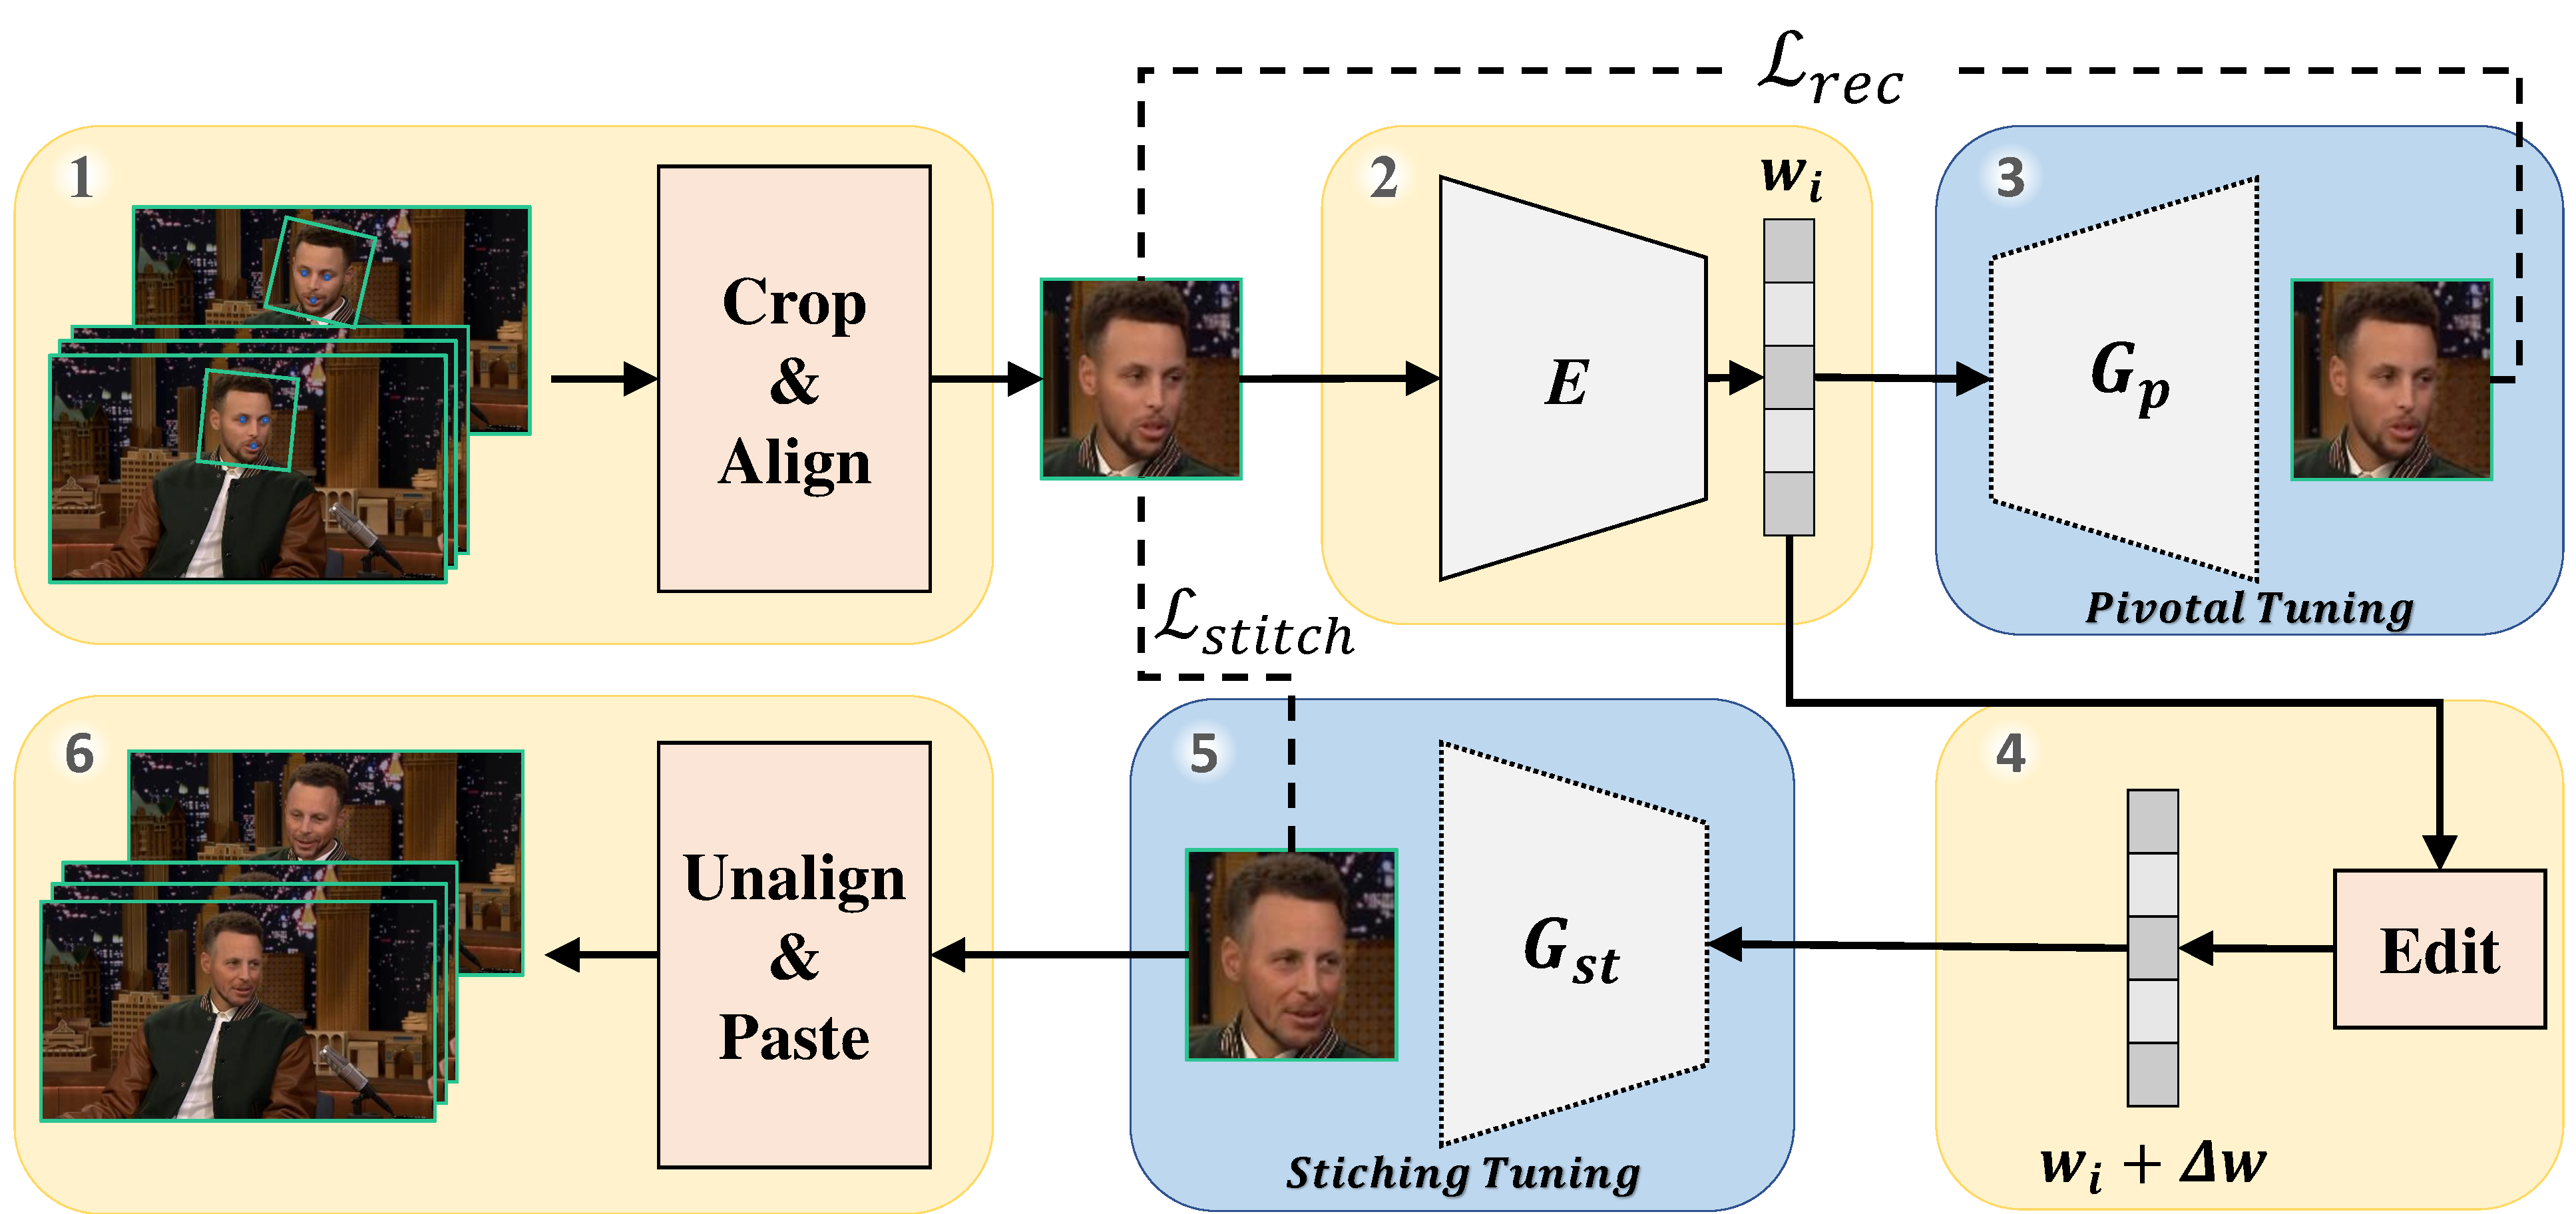
\includegraphics[width=0.97\linewidth]{resources/images/pipeline.pdf}
    % \vspace{-0.25cm}
    \caption{
    Our full video editing pipeline contains $6$ steps. $(1)$ Videos are split into individual frames. The face in each frame is cropped and aligned. $(2)$ Each cropped face is inverted into the latent space of a pre-trained StyleGAN2 model, using a pre-trained e4e encoder. $(3)$ The generator is fine-tuned using PTI across all video frames in parallel, correcting for inaccuracies in the initial inversion and restoring global coherence. $(4)$ All frames are edited by manipulating their pivot latent codes linearly, using a fixed direction and step-size. $(5)$ We fine-tune the generator a second time, stitching the backgrounds and the edited faces together in a spatially-smooth manner. $(6)$ We reverse the alignment step and paste the modified face into the video.
    }
    % \vspace{-0.1cm}
    \label{fig:pipeline}
\end{figure*}
\begin{figure}
\setlength{\tabcolsep}{0.5pt}
    \centering
    { \small 
\begin{tabular}{ccccc}
Original & e4e Encoding & $+$PTI & $+$Editing & $+$Stitching \\
\raisebox{-.32\totalheight}{
\includegraphics[width=0.2\columnwidth]{resources/images/pipeline_example/source_0010.jpeg}} &
\raisebox{-.32\totalheight}{
\includegraphics[width=0.2\columnwidth]{resources/images/pipeline_example/e4e_0010.jpeg}} &
\raisebox{-.32\totalheight}{
\includegraphics[width=0.2\columnwidth]{resources/images/pipeline_example/pti_0010.jpeg}} &
\raisebox{-.32\totalheight}{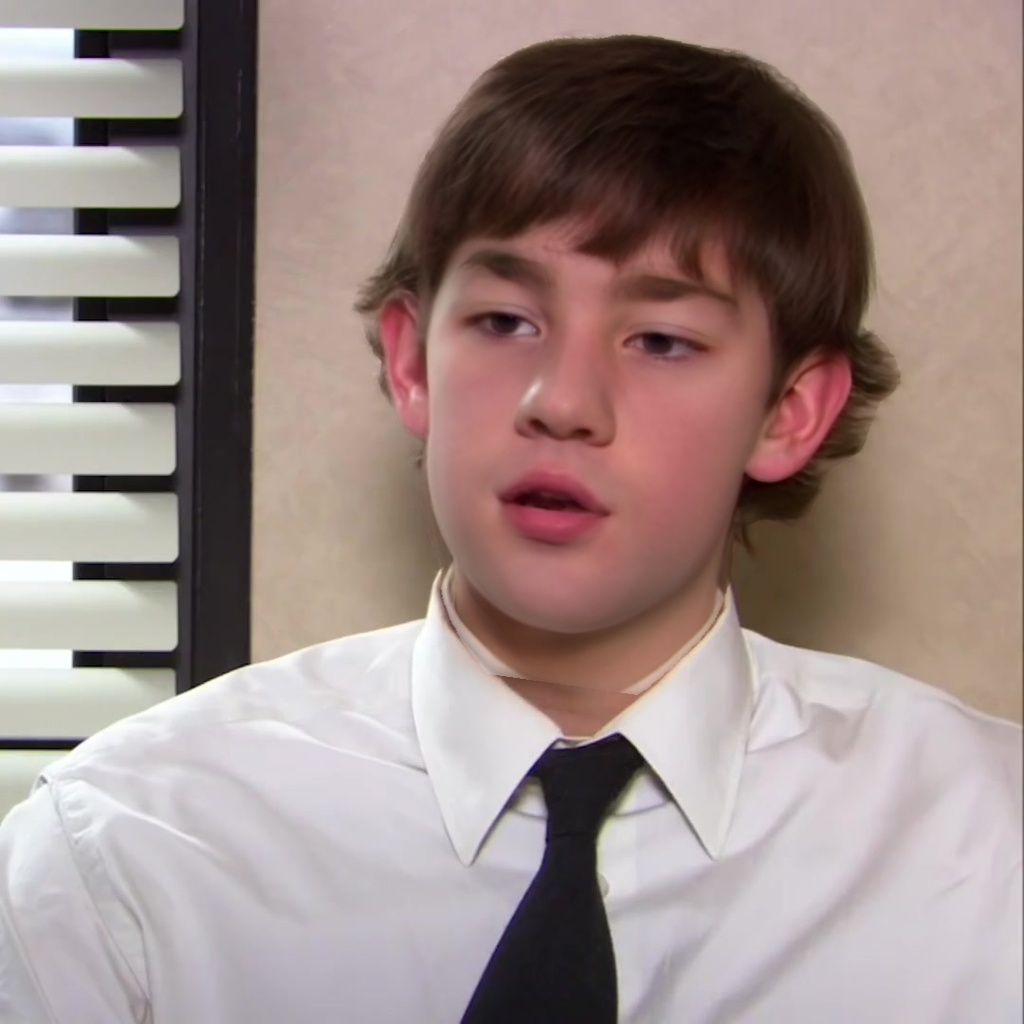
\includegraphics[width=0.2\columnwidth]{resources/images/pipeline_example/edit_0010.jpeg}} &
\raisebox{-.32\totalheight}{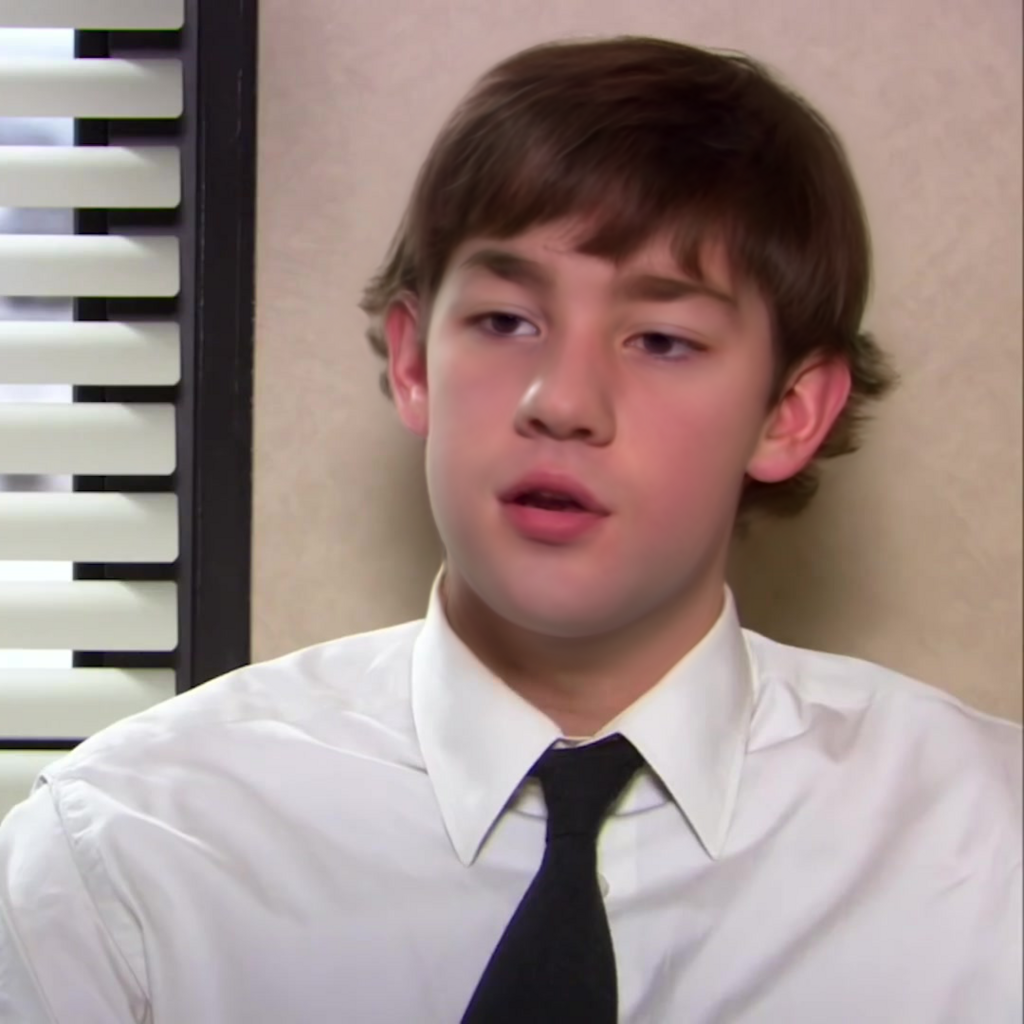
\includegraphics[width=0.2\columnwidth]{resources/images/pipeline_example/edit_stitching_10.png}} \\

\raisebox{-.32\totalheight}{
\includegraphics[width=0.2\columnwidth]{resources/images/pipeline_example/source_0015.jpeg}} &
\raisebox{-.32\totalheight}{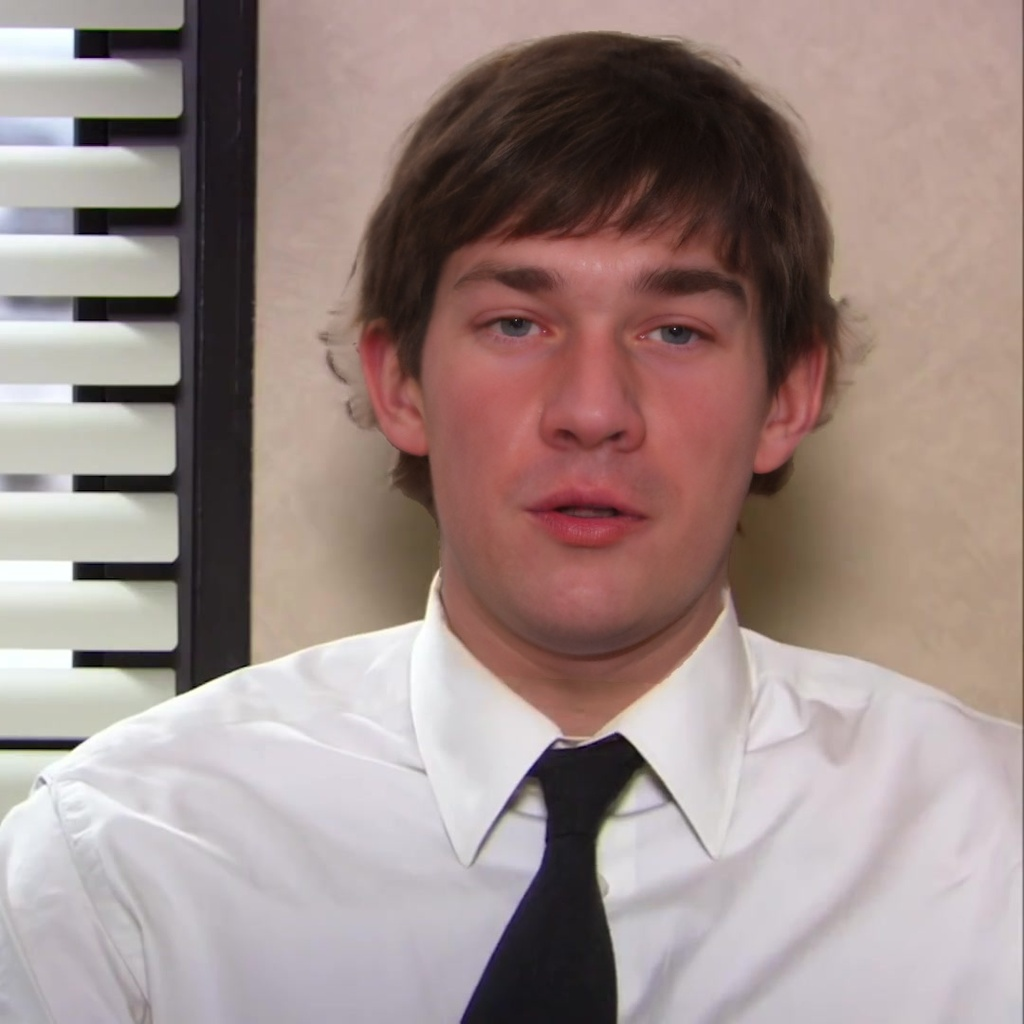
\includegraphics[width=0.2\columnwidth]{resources/images/pipeline_example/e4e_0015.jpeg}} &
\raisebox{-.32\totalheight}{
\includegraphics[width=0.2\columnwidth]{resources/images/pipeline_example/pti_0015.jpeg}} &
\raisebox{-.32\totalheight}{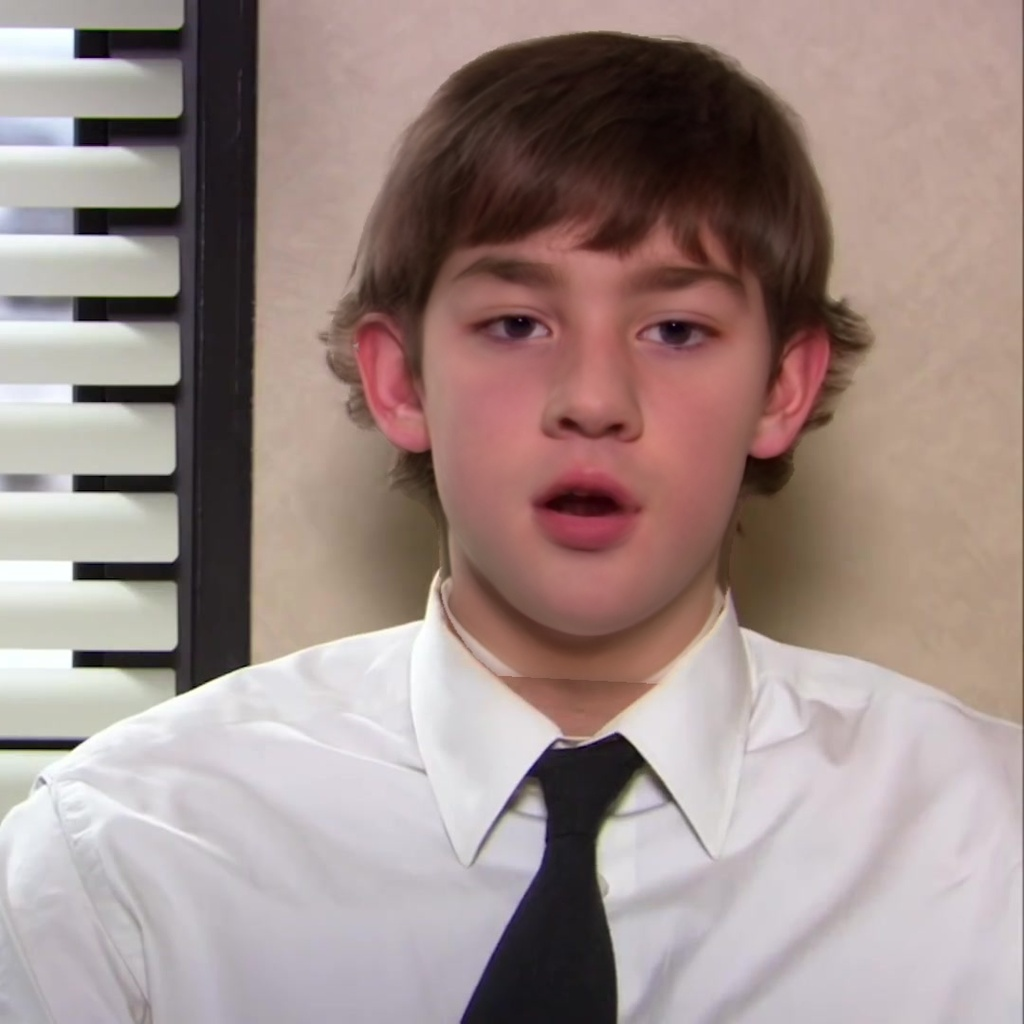
\includegraphics[width=0.2\columnwidth]{resources/images/pipeline_example/edit_0015.jpeg}} &
\raisebox{-.32\totalheight}{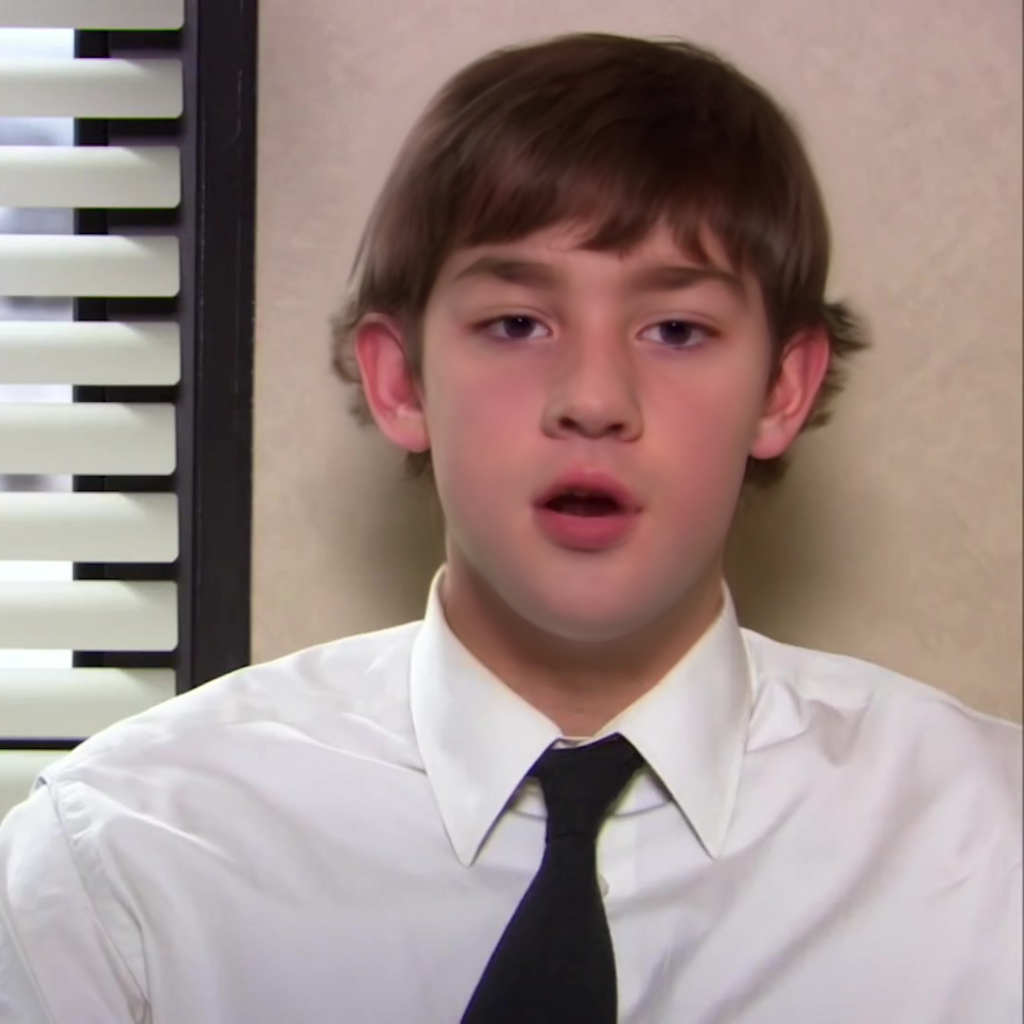
\includegraphics[width=0.2\columnwidth]{resources/images/pipeline_example/edit_stitching_15.png}} \\

\raisebox{-.32\totalheight}{
\includegraphics[width=0.2\columnwidth]{resources/images/pipeline_example/source_0020.jpeg}} &
\raisebox{-.32\totalheight}{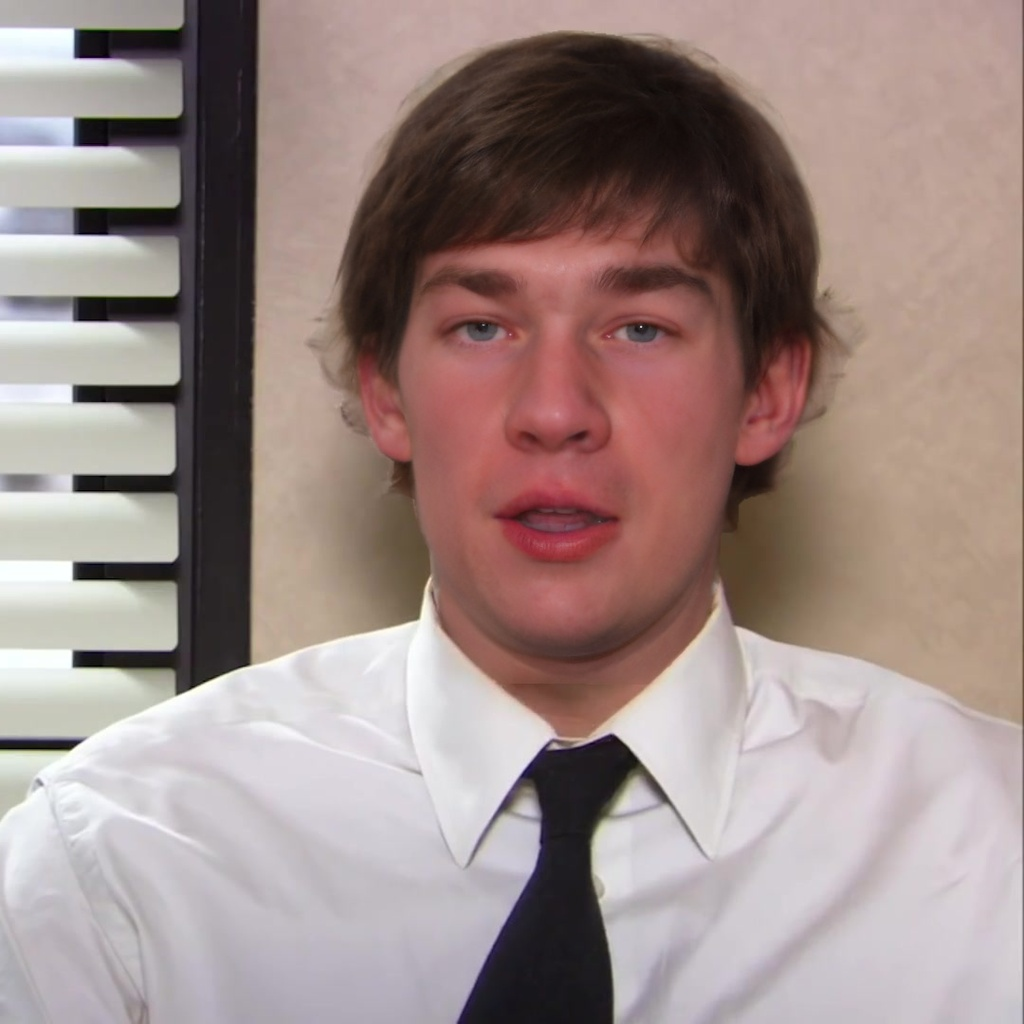
\includegraphics[width=0.2\columnwidth]{resources/images/pipeline_example/e4e_0020.jpeg}} &
\raisebox{-.32\totalheight}{
\includegraphics[width=0.2\columnwidth]{resources/images/pipeline_example/pti_0020.jpeg}} &
\raisebox{-.32\totalheight}{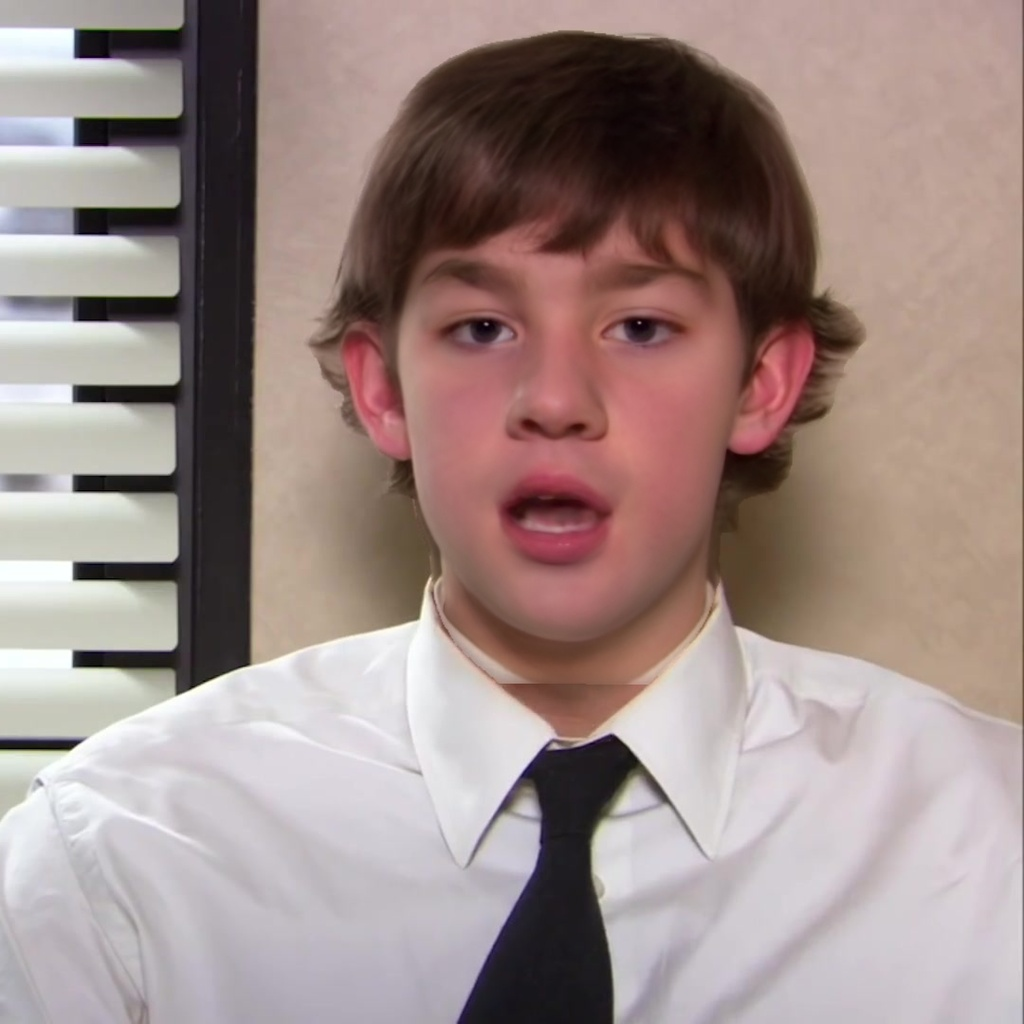
\includegraphics[width=0.2\columnwidth]{resources/images/pipeline_example/edit_0020.jpeg}} &
\raisebox{-.32\totalheight}{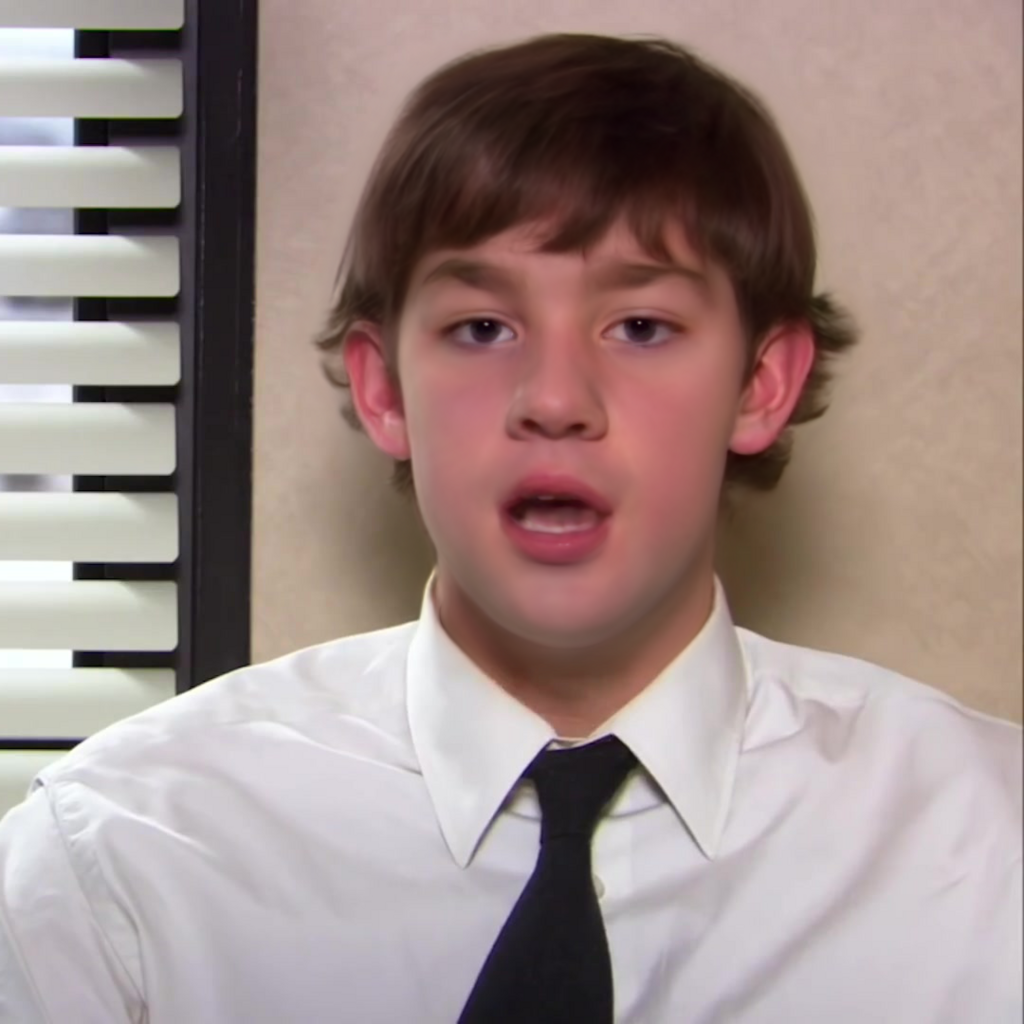
\includegraphics[width=0.2\columnwidth]{resources/images/pipeline_example/edit_stitching_20.png}} \\

\end{tabular}
}


\caption{Visualization of our full editing pipeline. In the left column, we show three frames extracted from the source video. In the following columns, we show intermediate results of our pipeline over the same three frames. Left to right: the encoder-inversion step, the PTI fine-tuning step, the pivot editing step, and finally our stitching procedure. When not applying our stitching procedure, we use a segmentation-mask based blending procedure~\shortcite{yao2021latent}. Note in particular the neck region, which displays considerable artifacts after the editing step which are then eliminated through our stitching-tuning approach. }

\label{fig:pipeline_example}
\end{figure}
